\documentclass[../main.tex]{subfiles}
\begin{document}
\section{Main results}
\label{sec:results}

The main results obtained from our model simulations and what it implicates for key macroeconomic variables are presented in this section. Furthermore, we compare our most important model simulations with actual data from Denmark.

\subsection{Decomposition of the NRI}
Our main result of this paper can be found in the decomposition of the NRI in Figure \ref{fig:decomp_NRI}. According to our model simulations, the NRI has fallen 1.8 percentage points from 1985-2020. The demographic transition accounts for half of the decline in the NRI, with the other half reflecting declining TFP growth in the world. Of the demographic changes, falling mortality is the most significant contribution accounting for 0.7 percentage points of the total decline in the NRI and low fertility accounting for 0.2 percentage points.\footnote{Despite a low interest rate, the economy is dynamically efficient, see \textcite{abel1989assessing}. The marginal product of capital is larger than the investment-to-capital ratio. In other words, the economy is investing less than it is getting from capital income.}

The dynamics between the demographic transition and the NRI are closely related to saving behaviour. Lower mortality risk translates into higher savings for households as they prefer to sustain consumption in retirement. Higher private savings lead to a higher capital accumulation resulting in a higher capital-to-labour ratio and a lower marginal product on capital which depresses the NRI. Lower fertility puts a further downward pressure on the NRI as it implies a shrinking workforce relative to the population. This will lead to an even higher capital-to-labour ratio, \textit{ceteris paribus}.

Recalling Figure \ref{fig:TFP_DepRatio_NetPublicDebt}, the slump in TFP growth from the late 1980s to the late 2000s has implied that agents' future income growth has somewhat stagnated. The expectation of a relatively lower labour income in the future has resulted in a higher incentive to accumulate private savings so households can finance consumption in the future. This has led to downward pressure on the NRI as the above-mentioned dynamics between savings and the NRI appear. 
The slight rebound post-2020, according to our model predictions, is mostly due to an expected increase in global TFP growth. These projections for the TFP growth are historically more uncertain than demographic projections. Consequently, this rebound relies on fluctuating and uncertain factors, which may be dwarfed by demographic factors that are highly likely to continue to play a profound role in pushing the real interest rate down. 

Interactions measure the impact of trading foreign assets. This effect is relatively small but is expected to affect the NRI positively from 2020-2040 due to an expected increase in net foreign asset position from a Danish perspective. A small capital outflow will result in a lower domestic capital accumulation and hence a higher marginal product on capital, contributing to a slightly higher NRI. Finally, the effect of low public debt in Denmark reflects negatively on the NRI, but the effect is quantitatively small.  

    \begin{figure}[H]
        \centering
        \caption{Decomposition of the fall in the Danish NRI}
        \label{fig:decomp_NRI}
        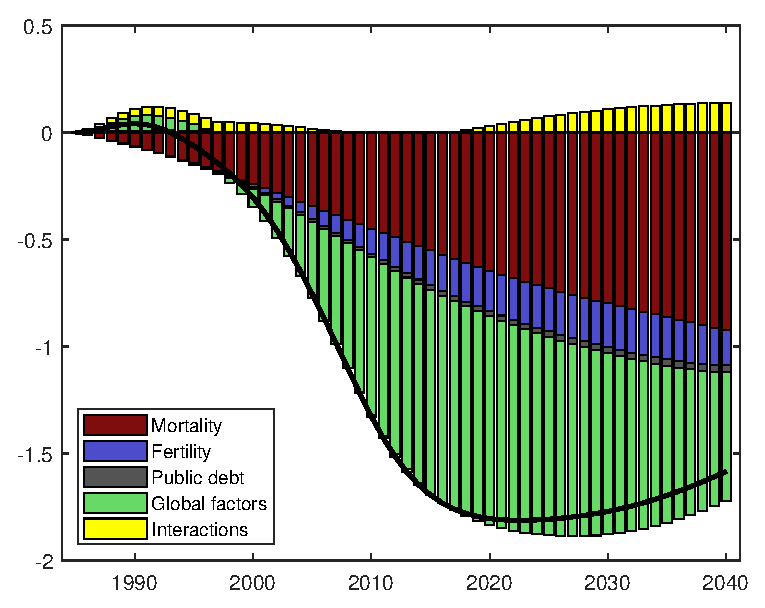
\includegraphics[]{Figures/Figure_6.eps}\\
            \begin{fignote}
            \textit{Note:} Levels express changes in percentage points from 1985. The decomposition is based in 1985 as simulations showed a stable NRI before going into the 1990s. Global factors combine the effects of TFP growth and foreign interest rate. Interactions cover the effect of international trade.
            \end{fignote}
    \end{figure}

\newpage
These findings have a direct link to the degree of households' preferences for consumption smoothing, $\sigma$. We impose the simple case of CRRA preferences with log-utility ($\sigma=1$) where income and substitution effects cancel out. However, if we assume that households are more willing to accept large differences in consumption between periods ($\sigma>1$), we expect to see a less dramatic fall in the NRI. This is because households will make fewer adjustments to saving profiles given a higher life expectancy or fall in TFP growth to sustain consumption in the future. On the contrary, if we assume households care more about consumption smoothing ($\sigma<1$), we would expect to see an even stronger decline in the NRI than we found in our baseline scenario. In this case, households will adjust savings more aggressively in response to a longer retirement period implying a stronger effect on the NRI. A meta-study by \textcite{havranek2015cross} combines estimates from 169 studies and find that a worldwide empirical measure of $\sigma$ is around 0.5, which would result in a steeper decline in the NRI than our results suggest.

\subsection{Other key macroeconomic variables}
The demographic transition's impact on key macroeconomic variables is illustrated in Figure \ref{fig:Baseline_model_sim}. As the Danish population ages, it causes a labour scarcity that is reflected in decreasing labour input per capita (Figure \ref{fig:Baseline_model_sim}\textcolor{blue}{A}), especially from the mid-2000s. The real wages per efficiency unit in Figure \ref{fig:Baseline_model_sim}\textcolor{blue}{B} increase from 1990 due to relatively low TFP growth in the world and starts to accelerate in the mid-2000s as a consequence of a lower labour input per capita. This leads to a higher capital-labour ratio shown in Figure \ref{fig:Baseline_model_sim}\textcolor{blue}{C}. A more capital intensive economy implies higher investments (Figure \ref{fig:Baseline_model_sim}\textcolor{blue}{D}). However, this development is relatively short-lived, as the investment-to-output ratio subsequently decreases after 2010 as the need for investment decreases due to a higher proportion of retirees. Unsurprisingly, the ageing of Danish society causes a saving boom as seen in Figure \ref{fig:Baseline_model_sim}\textcolor{blue}{E}. Finally, for a given retirement age of 65 and a fixed replacement rate of 42 percent, population ageing implies increasing taxes to finance future public pensions (Figure \ref{fig:Baseline_model_sim}\textcolor{blue}{F}).

\begin{figure}[H]
    \centering
    \caption{Baseline model simulation}
    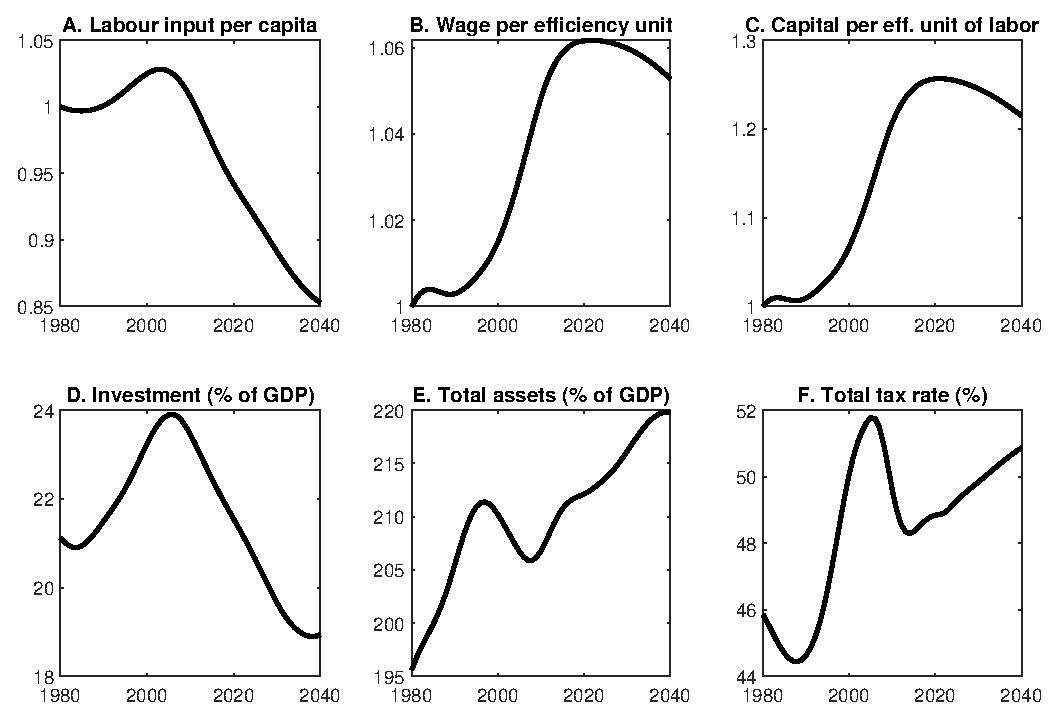
\includegraphics[scale=0.8]{Figures/Figure_7B.eps}
    \label{fig:Baseline_model_sim}
    \begin{fignote}
        \textit{Note:} Labour input per capita, wage per efficiency unit, and capital per efficiency unit of labour have been normalized to unity in 1980.
    \end{fignote}
\end{figure}
Compared to available data, our calibrated model seems to capture trends excellently. Hours worked per capita in Figure \ref{fig:predict_vs_data}\textcolor{blue}{A} are slightly off due to relatively large cohort sizes of post-war baby boomers reaching the age of late 50s to mid-60s that are attributed a relatively high productivity $z_j$ (recall Figure \ref{fig:Life_cycle}\textcolor{blue}{A}). The demographic transition and productivity slowdown cause a decline in GDP growth which is matched well by data in Figure \ref{fig:predict_vs_data}\textcolor{blue}{B}. The data series for net foreign assets is also matched reasonably well within our targeted period of 2000-2007. However, the model cannot capture cyclical movements post 2009. We don't consider this to be a major problem, as our focus is primarily on the macroeconomic development caused by structural changes (i.e. demographics in this case) rather than the cyclical reasons, which is beyond the scope of this paper.
\begin{figure}[H]
    \centering
    \caption{Predictions vs data}
    \label{fig:predict_vs_data}
    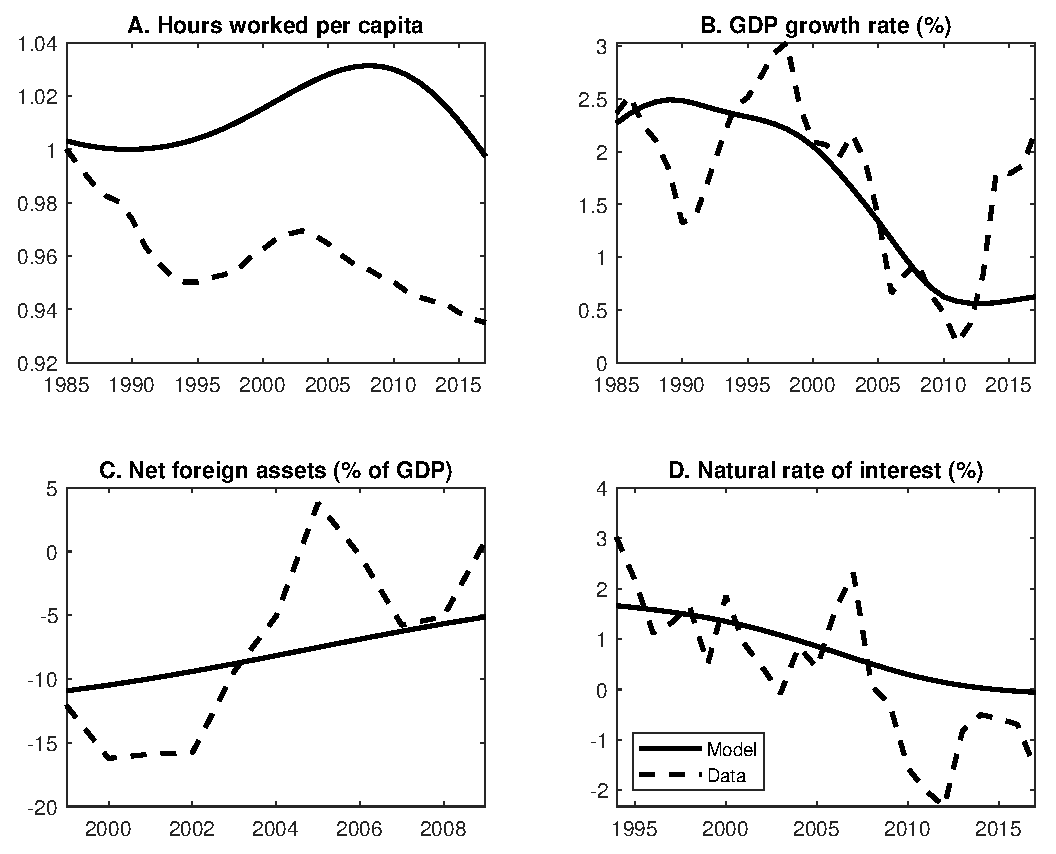
\includegraphics[scale=0.8]{Figures/Figure_8.eps}
    \begin{fignote}
        \textit{Note:} Data for GDP growth is taken from Statistikbanken, table NAN1, and smoothed by an 8 year-moving average. Net foreign assets is taken from \textcite{abildgren2017chart}. The real interest rate is Nationalbanken's \textit{diskonto} minus inflation (consumer price index), table DNRENTA and PRIS9 from Statistikbanken. Data for hours worked is taken from OECD and normalized to unity in 1985.
    \end{fignote}
\end{figure}



\end{document}